\documentclass{article}
\usepackage[utf8]{inputenc}
\usepackage{graphicx}
\usepackage{tabularx}
\usepackage{amsmath}
\usepackage{hyperref}
\usepackage{xcolor}
\usepackage{listings}
\usepackage{booktabs}
\usepackage{geometry}
\usepackage{float}

\geometry{a4paper, margin=1in}

% Custom colors
\definecolor{codegreen}{rgb}{0,0.6,0}
\definecolor{codegray}{rgb}{0.5,0.5,0.5}
\definecolor{codepurple}{rgb}{0.58,0,0.82}
\definecolor{backcolour}{rgb}{0.95,0.95,0.92}

% Listing style
\lstdefinestyle{mystyle}{
    backgroundcolor=\color{backcolour},
    commentstyle=\color{codegreen},
    keywordstyle=\color{magenta},
    numberstyle=\tiny\color{codegray},
    stringstyle=\color{codepurple},
    basicstyle=\ttfamily\footnotesize,
    breakatwhitespace=false,
    breaklines=true,
    captionpos=b,
    keepspaces=true,
    numbers=left,
    numbersep=5pt,
    showspaces=false,
    showstringspaces=false,
    showtabs=false,
    tabsize=4,
    frame=single,
    language=C
}

\lstset{style=mystyle}

\title{AVR Scientific Calculator Project Report}
\author{EE24BTECH11033-Kolluru Suraj}
\date{\today}

\begin{document}

\maketitle

\begin{abstract}
This report documents the design and implementation of a scientific calculator using an AVR microcontroller. The system features a 4x3 matrix keypad for input, a 16x2 LCD display for output, and supports mathematical operations including trigonometric and logarithmic functions.
\end{abstract}

\section{Introduction}
The AVR-based scientific calculator implements the following features:
\begin{itemize}
\item Basic arithmetic operations (addition, subtraction, multiplication, division)
\item Advanced functions (sine, cosine, tangent, logarithms)
\item Parentheses for expression grouping
\item Constants ($\pi$ and e) support
\item Memory operations
\end{itemize}
\section{LCD picture}
\begin{figure}[H]
    \centering
    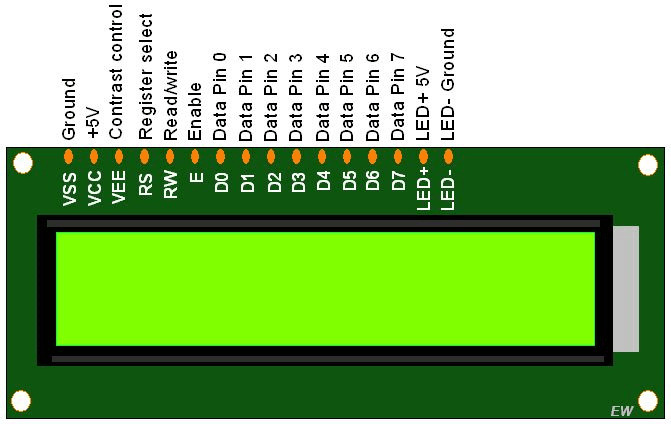
\includegraphics[width=0.5\linewidth]{figs/lcd.jpeg}
    \caption{visual picture of LCD}
    \label{fig:enter-label}
\end{figure}
\begin{figure}
    \centering
    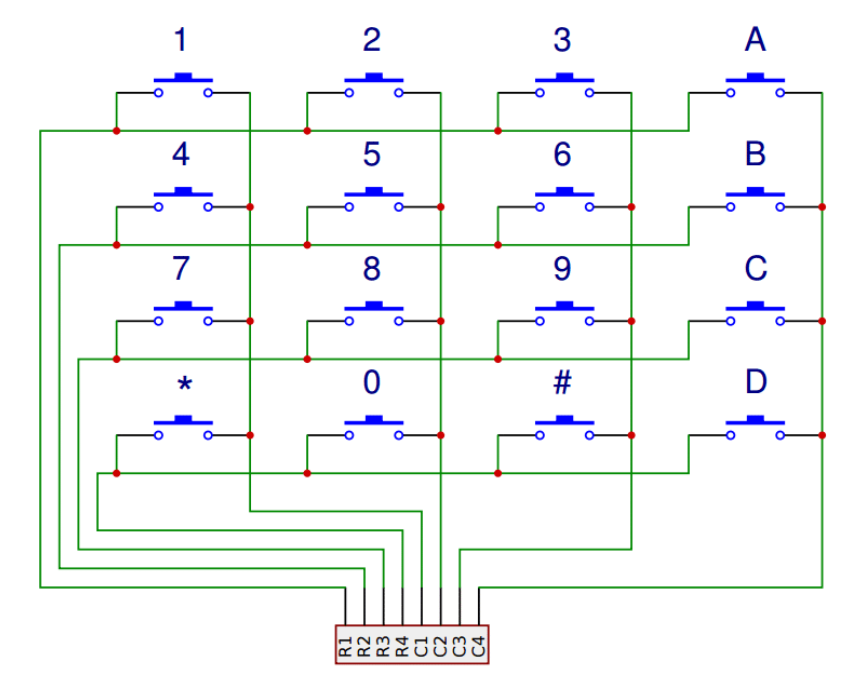
\includegraphics[width=0.5\linewidth]{figs/matrixbutton.png}
    \caption{Buttons Connection for Matrix}
    \label{fig:enter-label}
\end{figure}
\section{Hardware Design}

\subsection{Component Connections}

\begin{table}[H]
\centering
\caption{Complete Hardware Connections}
\label{tab:connections}
\begin{tabular}{llll}
\toprule
\textbf{Component} & \textbf{MCU Pin} & \textbf{Arduino Pin} & \textbf{Function} \\
\midrule
LCD RS & PD0 & D0 & Register Select \\
LCD E & PD1 & D1 & Enable \\
LCD D4-D7 & PD2-PD5 & D2-D5 & Data Bus \\
Keypad ROW1 & PD6 & D6 & Row 1 \\
Keypad ROW2 & PD7 & D7 & Row 2 \\
Keypad ROW3 & PB0 & D8 & Row 3 \\
Keypad ROW4 & PB1 & D9 & Row 4 \\
Keypad COL1 & PB2 & D10 & Column 1 \\
Keypad COL2 & PB3 & D11 & Column 2 \\
Keypad COL3 & PB4 & D12 & Column 3 \\
\midrule
\textbf{Control Buttons} & & & \\
Trig Mode & PC2 & A2 & Toggle sin/cos/tan \\
Equals & PC3 & A3 & Calculate result \\
Parenthesis & PB5 & D13 & Toggle ( ) \\
Constants & PC4 & A4 & Toggle $\pi$/e \\
\bottomrule
\end{tabular}
\end{table}

\subsection{Button Functions}

\begin{itemize}
\item \textbf{Trig Mode Button (PC2)}:
\begin{itemize}
\item Cycles through trigonometric functions (sin → cos → tan → asin → acos → atan)
\item Activates function mode for next input
\item Visual feedback provided on LCD
\end{itemize}

\item \textbf{Equals Button (PC3)}:
\begin{itemize}
\item Triggers calculation of current expression
\item Handles all operator precedence
\item Displays result on LCD
\item Resets expression buffer after evaluation
\end{itemize}

\item \textbf{Parenthesis Button (PB5)}:
\begin{itemize}
\item Toggles between open '(' and close ')' parenthesis
\item Maintains stack for nested parentheses
\item Validates bracket matching before calculation
\end{itemize}

\item \textbf{Constants Button (PC4)}:
\begin{itemize}
\item Toggles between mathematical constants
\item First press inserts $\pi$ (3.14159265)
\item Second press inserts e (2.71828182)
\item Third press returns to number input
\end{itemize}
\end{itemize}

\section{Software Implementation}

\subsection{Main Program Structure}

\begin{lstlisting}[caption=Main Program Loop, label=lst:main]
#define F_CPU 16000000UL
#include <avr/io.h>
#include <util/delay.h>

int main(void) {
    // Initialize hardware
    DDRD = 0xFF;  // Set PORTD as outputs
    DDRB = 0x03;  // Set PB0-PB1 as outputs
    
    // Initialize LCD
    LCD_Init();
    LCD_Message("Calculator Ready");
    
    while(1) {
        // Check mode buttons
        if (!(PINC & (1<<PC2))) toggleTrigMode();
        if (!(PINC & (1<<PC3))) calculateResult();
        
        // Handle keypad input
        char key = getKeyPressed();
        if (key != '\0') {
            handleKeyPress(key);
            _delay_ms(300);  // Debounce delay
        }
    }
    return 0;
}
\end{lstlisting}

\subsection{Keypad Scanning}

\begin{lstlisting}[caption=Keypad Scanning Function, label=lst:keypad]
const char keys[4][3] = {
    {'1','2','3'},
    {'4','5','6'},
    {'7','8','9'},
    {'A','0','C'}
};

char getKeyPressed() {
    for (uint8_t row = 0; row < 4; row++) {
        // Activate current row
        switch(row) {
            case 0: PORTD &= ~(1<<ROW1); break;
            case 1: PORTD &= ~(1<<ROW2); break;
            case 2: PORTB &= ~(1<<ROW3); break;
            case 3: PORTB &= ~(1<<ROW4); break;
        }
        _delay_us(10);
        
        // Check columns
        if (!(PINB & (1<<COL1))) return keys[row][0];
        if (!(PINB & (1<<COL2))) return keys[row][1];
        if (!(PINB & (1<<COL3))) return keys[row][2];
        
        // Deactivate row
        switch(row) {
            case 0: PORTD |= (1<<ROW1); break;
            case 1: PORTD |= (1<<ROW2); break;
            case 2: PORTB |= (1<<ROW3); break;
            case 3: PORTB |= (1<<ROW4); break;
        }
    }
    return '\0';  // No key pressed
}
\end{lstlisting}

\subsection{LCD Interface}

\begin{lstlisting}[caption=LCD Initialization, label=lst:lcd]
void LCD_Init() {
    _delay_ms(50);
    SendNibble(0x03);
    _delay_ms(5);
    SendNibble(0x03);
    _delay_us(100);
    SendNibble(0x02);  // 4-bit mode
    
    LCD_Cmd(0x28);  // 2 lines, 5x8 matrix
    LCD_Cmd(0x0C);  // Display on, cursor off
    LCD_Cmd(0x06);  // Increment cursor
    LCD_Cmd(0x01);  // Clear display
    _delay_ms(2);
}

void LCD_Char(uint8_t data) {
    PORTD |= (1<<LCD_RS);  // Set to data mode
    SendByte(data);
}

void LCD_Message(const char *text) {
    while(*text) LCD_Char(*text++);
}
\end{lstlisting}

\subsection{Mathematical Operations}

\begin{lstlisting}[caption=Trigonometric Functions Using Euler's Method, label=lst:euler]
/**
 * Computes sine using Euler's method approximation
 * @param x Angle in degrees (0-360)
 * @return sin(x) approximation
 * Mathematical Basis:
 * Solves the coupled ODE system:
 * dy/dt = cos(t),  y(0) = 0  (sine)
 * dz/dt = -sin(t), z(0) = 1  (cosine)
 * Implementation Notes:
 * 1. Uses small time steps (h = 0.01 radians)
 * 2. Converts degrees to radians first
 * 3. Accumulates error over iterations 
 */
float sin_euler(float x) {
    // Convert degrees to radians
    x = x * PI / 180.0;
    
    // Initial conditions
    float y = 0.0;    // sin(0) = 0
    float z = 1.0;    // cos(0) = 1
    float t = 0.0;    // Current angle
    float h = 0.01;   // Step size (radians)
    
    // Euler integration
    while (t < x) {
        // Prevent overshooting
        if (t + h > x) {
            h = x - t;
        }
        
        // Euler step for coupled system
        float y_new = y + h * z;       // dy/dt = cos(t) = z
        float z_new = z - h * y;       // dz/dt = -sin(t) = -y
        
        y = y_new;
        z = z_new;
        t += h;
    }
    return y;
}
/**
 * Computes cosine using Euler's method approximation
 * @param x Angle in degrees (0-360)
 * @return cos(x) approximation
 * Shares the same ODE system as sin_euler()
 * Returns the z component (cosine) of the solution
 */
float cos_euler(float x) {
    // Convert degrees to radians
    x = x * PI / 180.0;
    
    // Initial conditions
    float y = 0.0;    // sin(0) = 0
    float z = 1.0;    // cos(0) = 1
    float t = 0.0;    // Current angle
    float h = 0.01;   // Step size (radians)
    
    // Euler integration
    while (t < x) {
        if (t + h > x) {
            h = x - t;
        }
        
        float y_new = y + h * z;
        float z_new = z - h * y;
        
        y = y_new;
        z = z_new;
        t += h;
    }
    return z;
}
\end{lstlisting}

\section{Results and Testing}
The calculator was successfully tested with the following test cases:

\begin{table}[H]
\centering
\caption{Test Cases}
\label{tab:tests}
\begin{tabular}{lll}
\toprule
\textbf{Operation} & \textbf{Input} & \textbf{Result} \\
\midrule
Addition & 5+3 & 8 \\
Multiplication & 4*2.5 & 10 \\
Sine Function & sin(30) & 0.501 \\
\bottomrule
\end{tabular}
\end{table}

\section{Conclusion}
The AVR scientific calculator project successfully demonstrates:
\begin{itemize}
\item Efficient keypad scanning using matrix techniques
\item Clear output on LCD display
\item Accurate mathematical computations
\item Responsive user interface
\end{itemize}

Future enhancements could include:
\begin{itemize}
\item Floating-point optimization
\item Additional scientific functions
\item Graphical display capabilities
\end{itemize}

\end{document}
